\pdfminorversion=4
%----------------------------------------------------------------------------------------
%	FELIX NEWCOMMANDS
%----------------------------------------------------------------------------------------
% equalsign with space
\def\eq{\ensuremath{&\quad=\quad}}
% unit vector
\def\uvec#1{\ensuremath{\hat{\mathbf{e}}_{\textup{#1}}}}
% The number `e'.
\def\eu{\ensuremath{\mathrm{e}}}
% The imaginary unit.
\def\iu{\ensuremath{\mathrm{i}}}
% The differential operator.
\def\du{\ensuremath{\mathrm{d}}}
% kappax0
\def\kap{\ensuremath{\mathrm{\kappa_{\textup{x}0}}}}

%----------------------------------------------------------------------------------------
%	PACKAGES AND OTHER DOCUMENT CONFIGURATIONS
%----------------------------------------------------------------------------------------

\documentclass[8pt,aspectratio=169]{beamer}
\usetheme{metropolis}
%\usepackage[sfdefault]{FiraSans}
\usepackage[sfdefault]{sourcesanspro}

\usepackage[utf8]{inputenc} % Required for inputting international characters
\usepackage[T1]{fontenc} % Output font encoding for international characters

\usepackage{graphicx}
\usepackage{color, colortbl}

\usepackage{booktabs} % necessary for undliner, midrule, ...
%\usepackage{libertine}
%\usepackage[libertine,cmintegrals,cmbraces,vvarbb]{newtxmath}
%\usepackage[makeroom]{cancel}
%\usepackage{xcolor}
%\newcommand\Ccancel[2][black]{\renewcommand\CancelColor{\color{#1}}\xcancel{#2}}

\usepackage[backend=bibtex, style=numeric, natbib=true, isbn=false, backref=true, sorting=none, url=false]{biblatex} % Use the bibtex backend with the authoryear citation style (which resembles APA)

\addbibresource{bibliography.bib} % The filename of the bibliography

\usepackage[autostyle=true]{csquotes} % Required to generate language-dependent quotes in the bibliography

\usepackage[export]{adjustbox} % The adjustbox package allows you to add alignment keys to \includegraphics
\usepackage{siunitx}
\usepackage[labelformat=empty, font=footnotesize]{caption}
\usepackage{tikz}
%----------------------------------------------------------------------------------------
%	BEAMER TEMPLATE
%----------------------------------------------------------------------------------------
\definecolor{darkblue}{RGB}{35, 55, 59}
\definecolor{pitchblack}{RGB}{0, 0, 0}
\definecolor{lightbeige}{RGB}{255, 251, 241}
\definecolor{mediumgray}{RGB}{183, 183, 183}

%\beamertemplatenavigationsymbolsempty % no navigation
\setbeamercolor{frametitle}{bg=white, fg=darkblue}
\setbeamercolor{background canvas}{bg=white}
%\setbeamerfont{frametitle}{size=\small}

\usepackage{hyperref}

\begin{document} 
	
\begin{frame}\pdfbookmark{Title page}{Title page}
\begin{center}
\begin{minipage}{0.25\textheight}
\includegraphics[width = \linewidth]{images/hzblogo/hzb_logo_cmyk.pdf}
\end{minipage}
\hspace{10pt}
\begin{minipage}{0.25\textheight}
\includegraphics[width = \linewidth]{images/hulogo/husiegel_bw-eps-converted-to.pdf}
\end{minipage}
\vfill\vfill
{\bfseries {\large Optimization of the BESSY II optics for the VSR project - }\\Increase the installation length for the VSR cryomodule in the T2 section of the BESSY~II storage ring}
\vfill\vfill

\begin{small}
\begin{minipage}[t]{0.42\textwidth}
\begin{flushleft}
\emph{Author:}\\
Felix \textsc{Andreas}
\end{flushleft}
\end{minipage}
\begin{minipage}[t]{0.42\textwidth}
\begin{flushright}
\emph{Supervisor:} \\
Prof. Dr. Andreas \textsc{Jankowiak}\\Dr. Paul \textsc{Goslawski}
\end{flushright}
\end{minipage}
\vfill
23.10.2017
\end{small}
\end{center}
\end{frame}

\begin{frame}{Table of contents}
	\setbeamertemplate{section in toc}[sections numbered]
	\tableofcontents[hideallsubsections]
\end{frame}


\section{Motivation}

\begin{frame}{BESSY II - A third generation light source}
	\begin{minipage}{0.6\linewidth}
\begin{figure}
	\includegraphics[height = 0.85\textheight]{images/01-BESSY-II-floor-plan-VSR-anno.pdf}
	\caption[Floor plan of synchrotron light source BESSY II.]{Floor plan of synchrotron light source BESSY II~\cite{Rubrecht_PhD}.}
	\label{fig:Bessy2-plan}
\end{figure}
\end{minipage}
\begin{minipage}{0.35\linewidth}
\begin{table}
	\centering
	\footnotesize
	\caption{Parameters of the BESSY II storage ring.}
	\begin{tabular}{ll}
\toprule
\textbf{Parameter}  &  \textbf{Value}\\
\midrule
nominal energy & 1.7\,GeV\\
circumference & 240\,m\\
RF-frequency & 500\,MHz\\
revolution time & 800\,ns\\
beam current & 300\,mA\\
number of cells & 16\\
number of bending magnets & 32\\
bending radius & 4.361\,m\\
beamlines & $\approx$ 50\\
\bottomrule
\end{tabular}

	\label{tab:mostimportantparameter}
\end{table}

\begin{table}
	\centering
	\footnotesize
	\caption{Bunch length $\sigma_\textup{z}$ - BESSY II vs BESSY VSR~\cite{vsrstudy}.}
	\begin{tabular}{lr}
\toprule
& \textbf{Bunch length} $\sigma_\textup{z} /$ ps\\
\midrule
BESSY II & 15 \\
BESSY II low alpha & 3 \\
\midrule
BESSY VSR short bunch & 1.7\\
BESSY VSR long bunch & 15\\
\bottomrule
\end{tabular}
\end{table}
\end{minipage}
\end{frame}





\begin{frame}{The VSR-cryomodule in the T2 straight}
	\begin{figure}
		\centering
		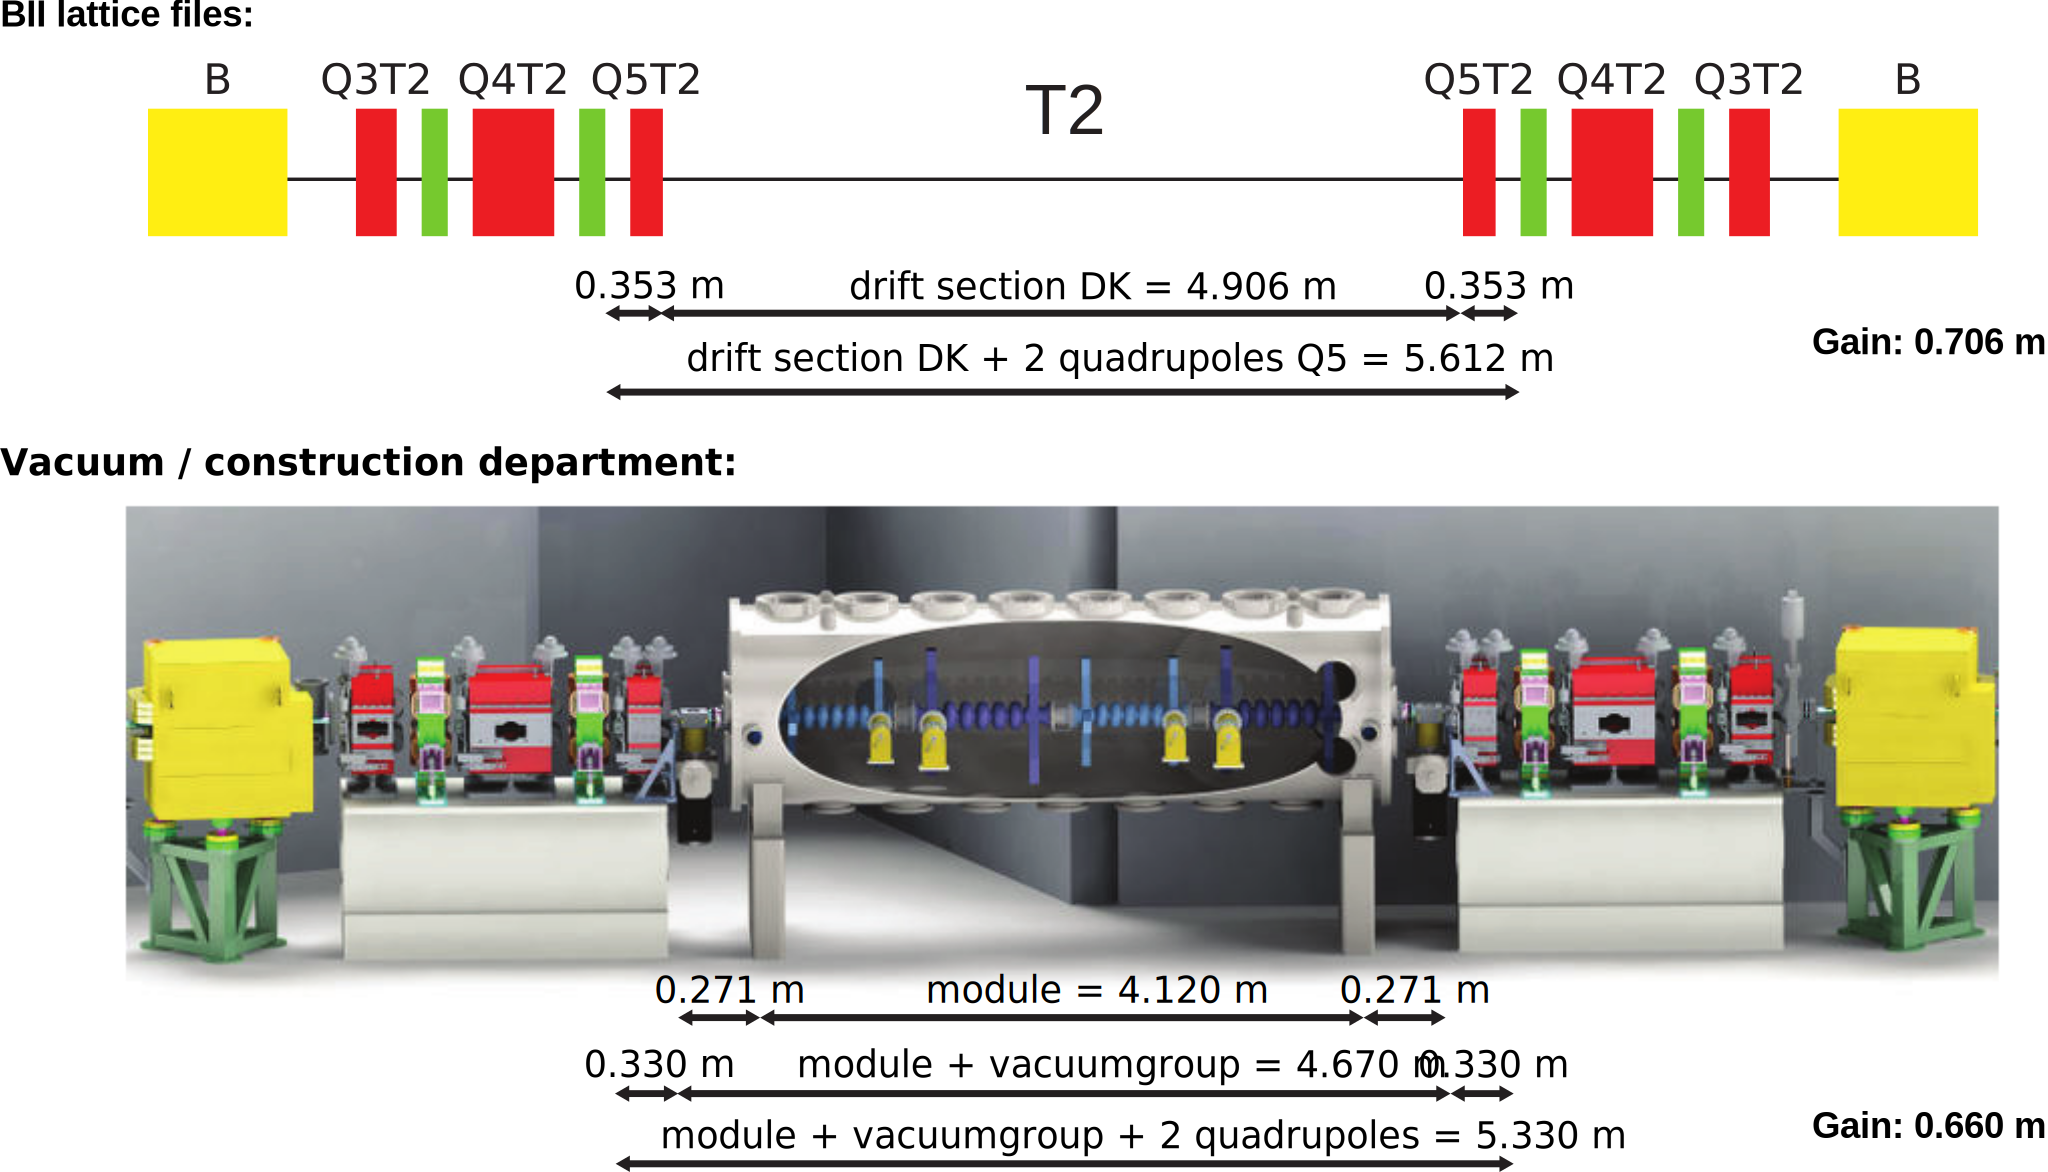
\includegraphics[width = 0.85\linewidth]{images/01-cavity-in-T2.pdf}
		\caption[The cryomodule and the magnets of the T2 section.]{The cryomodule and the magnets of the T2 section (dipole-yellow, quadruple-red, sextupole-green).}
		\label{fig:cavity-in-T2}
	\end{figure}
\end{frame}


\section{Transverse linear beam dynamics in circular accelerators}


\begin{frame}{Transverse linear beam dynamics in circular accelerators}
The equations of motion for a charged particle in a magnetic field in linear order
\begin{align}
u''(s) + K(s) u(s) = 0 &&&\quad \overset{\text{Floquet's theorem}}{\Rightarrow} \quad &&u(s) = \sqrt{\epsilon} \sqrt{\beta(s)} \cos(\psi(s) + \psi_0) \\[10pt]
\psi(s) = \int_0^s \frac{d \bar{s}}{\beta(\bar{s})} &&&\quad \: \, \, \overset{\text{one revolution}}{\Rightarrow} \quad &&Q = \frac{1}{2 \pi}\int_s^{s+C} \frac{d \bar{s}}{\beta(\bar{s})} 
\label{betatronphase}\end{align}

\begin{figure}
	\centering
	\includegraphics[width = 0.8\textwidth]{images/03-envelope.pdf}
	\caption[Envelope of a particle beam.]{The envelope of a particle beam at the example of a FODO cell. The betatron oscillation for 33 electrons with an emittance of 5 nm rad is shown in the right graphic.}
	\label{fig:envelope}
\end{figure}

\end{frame}

\begin{frame}{Transverse linear beam dynamics in circular accelerators II}
\begin{figure}
	\centering
	\includegraphics[width = .45\textwidth]{images/03-dispersion.pdf}
	\caption{Momentum dispersion in a dipole magnet.}
	\label{fig:dispersion}
\end{figure}
The dispersion function
\begin{equation}\begin{aligned}[b]
\eta(s) = \frac{\du u(s)}{\du \delta}
\end{aligned}\label{dudispersionfunction}\end{equation}
\begin{equation}\begin{aligned}[b]
u(s) &= u_{\beta}(s) + u_\delta(s) = u_{\beta}(s) + \eta(s) \delta
\end{aligned}\label{dispersivemotion}\end{equation}
The momentum compaction factor
\begin{equation}\begin{aligned}[b]
\alpha_\textup{c} = \frac{\Delta C_\delta/ C_\beta}{\delta} \quad \text{with} \quad C = C_\beta + \Delta C_\delta
\end{aligned}\label{momentumcompationfactor}\end{equation}
\begin{equation}\begin{aligned}[b]
\alpha_\textup{c} = \frac{1}{C_0} \int_0^{C_0} \kap(s) \eta(s) \du s 
\end{aligned}\label{momentumcompationfactor2}\end{equation}


\end{frame}






\section{The BESSY II storage ring lattice}


\begin{frame}{The Design lattice from 1996}
\begin{minipage}{0.8\linewidth}
\begin{figure}
\centering
\includegraphics[height = 0.65\textheight]{images/04-design-lattice-def.pdf}
\caption{The design lattice of the BESSY II storage ring.}
\label{fig:design-lattice}
\end{figure}
\end{minipage}
\begin{minipage}{0.18\linewidth}
\begin{table} 	
\centering
\footnotesize
%\caption{The quadrupole strengths of the design lattice.}
\begin{tabular}{lr}
\toprule
\textbf{Magnet} & k / m$^{-2}$\\
\midrule
Q1	& +2.45190 \\
Q2	& -1.89757\\
Q3D	& -2.02025\\
Q4D & +1.40816\\
Q3T & -2.46319\\
Q4T & +2.62081\\
Q5T & -2.60000\\
\bottomrule
\end{tabular}


\label{tab:magnetsstrengthsdesignlattice}
\end{table}
\end{minipage}
\end{frame}

\begin{frame}{The design lattice and the current standard lattice}
	\begin{figure}
		\centering
		\includegraphics[width = \linewidth]{images/04-design-vs-2017-lattice.pdf}
		\caption{Comparison between the design lattice and the current standard lattice (2017).}
		\label{fig:design-vs-2017-lattice}
	\end{figure}

\end{frame}




\begin{frame}{Requirements for new optics - Transverse multibunch instabilities}
	As stated in~\cite[p.~79]{Rubrecht_PhD} the transverse cavity impedances
	\begin{align}
	Z_{\textup{th}}^{\perp}(\tau_{\textup{d}}^{-1}) = \frac{\tau_{\textup{d}}^{-1}}{\beta} \frac{4 \pi E / e}{\omega_{\textup{rev}} I_{\textup{DC}}}
	\end{align}
	scale directly with the value of the beta function and could drive transverse multibunch instabilities. Therefore a beta function below 4\,m is required.
\begin{figure}
	\centering
	\includegraphics[width = 0.75\textheight]{images/04-betafunctioninT2.pdf}
	\caption[The horizontal and vertical betafunctions $\beta_{\textup{x,y}}$ in the T2 sections.]{The horizontal and vertical beta functions $\beta_{\textup{x,y}}$ in the T2 sections (based on~\cite{Rubrecht_PhD}).}
	\label{fig:betafunctioninT2}
\end{figure}
\end{frame}


\begin{frame}{The beta functions at the cyromodule}
The beta function at distance $s$ to a symmetry point can be calculated by:
\begin{align}
\beta(s) = \beta^* + \frac{s^2}{\beta^*}
\end{align}
\begin{figure}
\centering
\includegraphics[width = 0.75\textheight]{images/04-betafunction_in_cavity_def.pdf}
\caption[The maximal and average beta function within the cavity in dependence of the minimal beta function $\beta^*$.]{The maximal and average beta function within the cavity in dependence of the minimal beta function $\beta^*$ (based on~\cite{Ries, goslawski}).}
\label{fig:optimalbeta}
\end{figure}
\end{frame}

\section{Simulations of the new optics and verification at the machine}

\begin{frame}{First approach to turn off the Q5T2 magnets}
\begin{figure}
	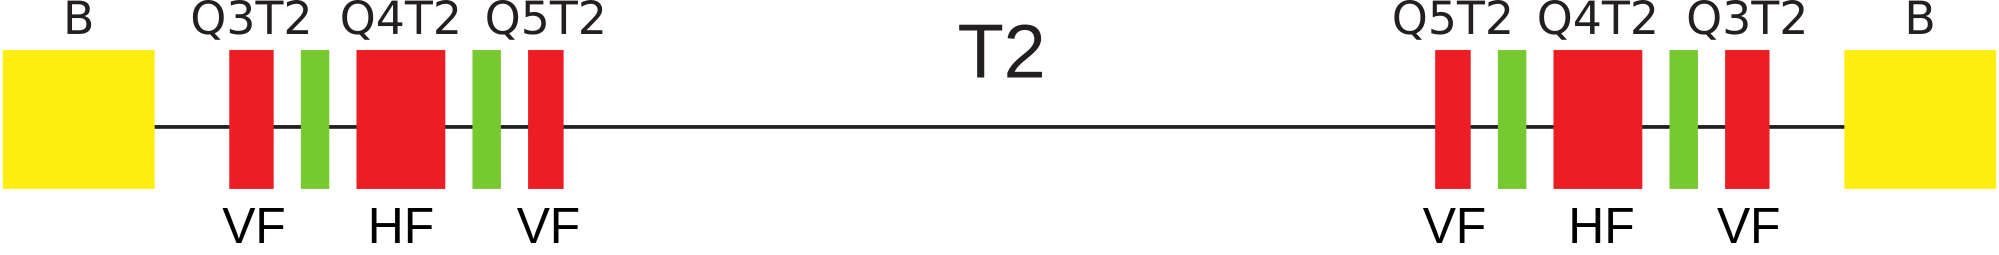
\includegraphics[width = 0.65\textwidth]{images/01-cavity-in-T2_def.pdf}
%	\caption{The T2 section of the BESSY~II storage ring.}
\end{figure}
\begin{enumerate}
\item Test how much the Q5T2 can be reduced without chancing any other magnet.
\item[$\Rightarrow$] The beam was lost at about 94\,\% of the initial value.
\vspace{8pt}
\item Compensate the vertical focusing Q5T2 by increasing the vertical focusing Q3T2.
\item[$\Rightarrow$] First allowed to reduce the Q5T2 slightly more, but lead then to the loss of the beam.
\vspace{8pt}
\item Compensate the vertical focusing Q5T2 by decreasing the horizontal focusing Q4T2.
\item[$\Rightarrow$] Achieved a working machine with switched of Q5T2 and an injection efficiency of about 20\,\%.
\end{enumerate}

\begin{table}[h!]
	\centering
	\footnotesize
	\caption{Changes in ampere of the quadrupoles in the T2 section compared to the standard BESSY II values}
	\begin{tabular}{lrrr}
\toprule
\textbf{signal}         &      \textbf{saved value} / A  &       \textbf{present value} / A & \textbf{factor} \\
\midrule
Q3PT2R:set      &                226.5832  &         219.7057 & 1.031\\
Q4PT2R:set      &                 189.587      &      246.5637 & 0.769\\
Q5PT2R:set     &                    18.25       &       227.68 & 0.080\\
Q5PT2R:stat1    &                     OFF       &           ON & -\\
\bottomrule
\end{tabular}

	\label{tab:first_approach}
\end{table}
\end{frame}


\begin{frame}{Limits of the lattice stability - FODO cell}
	The beta function for a periodic lattice:
	\begin{equation}\begin{aligned}[b]
	\beta(s) &\quad=\quad \frac{2 R_{12}}{\sqrt{2 - R_{11}^2 - 2 R_{12} R_{21} - R_{22}^2}}  \\
	\end{aligned}\label{twissperodicitycondition5}\end{equation}
\begin{figure}	
	\includegraphics[height = 0.6\textheight]{images/05-necktie-plot.pdf}
	\includegraphics[height = 0.6\textheight]{images/05-limits-of-FODOcell.pdf}	
	\caption{Limits of the FODO lattice stability.}
	\label{fig:necktieplot}
\end{figure}
\end{frame}


\begin{frame}{Limits of the lattice stability - BESSY~II}
	\begin{minipage}{0.4\linewidth}
		\begin{figure}
			\includegraphics[width = 0.75\textwidth]{images/05-stability-all_def.pdf}
			\caption{The lattice stability for BESSY II.}
			\label{fig:stabilitybessy2}
		\end{figure}
	\end{minipage}
	\begin{minipage}{0.59\linewidth}
		\begin{figure}
		\includegraphics[width = \textwidth]{images/05-bessy2-stability-Q3T2.pdf}
		\caption{Instability of the BESSY II storage ring lattice by the changing of the Q3T2.}
		\end{figure}
	\end{minipage}
\end{frame}


\begin{frame}{Optimization by minimization of a scalar function}
\metroset{block=fill} \footnotesize
\begin{minipage}[t]{0.44\linewidth}
	\begin{figure}
		\includegraphics[width = \textwidth]{images/04-stability-plot-bessy2_Q3_vs_Q4_Q5_off_betamaxvalue.pdf}
		\caption{Maximum value of the beta function with switched off Q5T2.}
	\end{figure}
	\textbf{Two conditions:}
	\begin{itemize} \footnotesize
		\item[1] The initial values must be in a stable area.
		\item[2] Optimization methods which does not need the derivative.
	\end{itemize}
\end{minipage}
\begin{minipage}[t]{0.55\linewidth}
\textbf{Three repetition of the Nelder-Mead algorithm:}
	\begin{block}{Step 1: Turn off the Q5T2}	
		\begin{equation}\begin{aligned}[b]
		f_1 = 10 \cdot ({k_{\textup{Q5T2}}})^{\frac{1}{4}} + \frac{\beta_{\textup{max}}}{\beta_{\textup{max,ref}}} + \frac{\overline{\beta}_{\textup{x,rel}} + \overline{\beta}_{\textup{y,rel}}}{2} \; \text{with} \; \overline{\beta}_{\textup{u,rel}} = \frac{1}{L} \int_{0}^{L} \du s \frac{\beta_{\textup{u}}}{\beta_{\textup{u,ref}}}
		\end{aligned}\label{function1}\end{equation}
	\end{block}
	
	\begin{block}{Step 2: Optimize the beta functions}
		\begin{equation}\begin{aligned}[b]
		f_2 =  \frac{\beta_{\textup{max}}}{\beta_{\textup{max,ref}}} + \frac{\overline{\beta}_{\textup{x,rel}} + \overline{\beta}_{\textup{y,rel}}}{2}
		\end{aligned}\label{function2}\end{equation}
	\end{block}
	
	\begin{block}{Step 3: Correct the tunes}
		\begin{equation}\begin{aligned}[b]
		f_3 = \frac{\beta_{\textup{max}}}{\beta_{\textup{max,ref}}} +  \frac{\overline{\beta}_{\textup{x,rel}} + \overline{\beta}_{\textup{y,rel}}}{2}  + 10 \cdot \left(|Q_{\textup{x}} - Q_{\textup{x,ref}}| +|Q_{\textup{y}} - Q_{\textup{y,ref}}|\right)
		\end{aligned}\label{function3}\end{equation}
	\end{block}
\end{minipage}
\end{frame}

\begin{frame}{Overview of the solutions with existing hardware}
	\begin{minipage}{0.49\linewidth}
		\begin{table}\small \begin{tabular}{ll}
\toprule
\textbf{Version}  &  \textbf{Used quadrupoles}\\
\midrule
V1   & T2   \\
V2   & D2, T2, D3    \\
V3   & T1, D2, T2, D3, T3   \\
V4   & D1, T1, D2, T2, D3, T3, D4   \\
V5   & T8, D1, T1, D2, T2, D3, T3, D4, T4   \\
Vall & all quadrupoles\\
\bottomrule
\end{tabular}
 \end{table}
	\end{minipage}
	\begin{minipage}{0.5\linewidth}
		\begin{figure} \includegraphics[height = 0.95\textheight, trim={0 0 0 0},clip]{images/05-V-versions-comparison_def.pdf} \end{figure}
	\end{minipage}
\end{frame}


\begin{frame}{Local solutions: V1}
Using only the magnets in the T2 section to compensate the turn off of the Q5T2.
\begin{table}[htbp!]
	\tiny
	\caption{Output of the minimization method for the local compensation V1.}
	\begin{tabular}{llrrrrr}
	\toprule
	{} & \textbf{Magnets} &  \textbf{Initial} &  \textbf{Final} &  \textbf{Difference} &  \textbf{Factor} & \textbf{Factor (exp.)} \\
	\midrule
	1 &        Q5PT2R    &            -2.588 &           0.000 &                2.588 &           -0.000 & 0.080 \\
	2 &        Q4PT2R    &             2.579 &           2.032 &               -0.547 &            0.788 & 0.769 \\
	3 &        Q3PT2R    &            -2.455 &          -2.630 &               -0.174 &            1.071 & 1.031\\
	\bottomrule
\end{tabular}\\
\begin{tabular}{rrrrrr}
\toprule
 $Q_{\textup{x}}$ / kHz &  $Q_{\textup{y}}$ / kHz &  $\beta_{\textup{x,max}}$ / m &  $\beta_{\textup{y,max}}$ / m &  $\overline{\beta}_{\textup{x,rel}}$ / m &  $\overline{\beta}_{\textup{y,rel}}$ / m \\
\midrule
                1060.54 &                  907.38 &                         32.34 &                         54.57 &                                     1.08 &                                     1.43 \\
\bottomrule
\end{tabular}

	\label{V1results}
\end{table}
\begin{figure}
	\includegraphics[width = \textwidth]{images/05-V1-comparison_def.pdf}
	\caption{Comparison of the V1 lattice (solid) with the current standard lattice (dashed).}
	\label{fig:V1-comaprison2}
\end{figure}

\end{frame}



\begin{frame}{Local solutions: V2}
\begin{table}[htbp!]

	\tiny
	\caption{Output of the minimization method for the extended local compensation V2.}
	\begin{tabular}{rrrrrr}
\toprule
 $Q_{\textup{x}}$ / kHz &  $Q_{\textup{y}}$ / kHz &  $\beta_{\textup{x,max}}$ / m &  $\beta_{\textup{y,max}}$ / m &  $\overline{\beta}_{\textup{x,rel}}$ / m &  $\overline{\beta}_{\textup{y,rel}}$ / m \\
\midrule
                1060.54 &                  907.39 &                         26.89 &                         33.58 &                                     1.01 &                                     1.13 \\
\bottomrule
\end{tabular}
\\\begin{tabular}{llrrrr}
\toprule
{} & \textbf{Magnets} &  \textbf{Initial} &  \textbf{Final} &  \textbf{Difference} &  \textbf{Factor} \\
\midrule
1 &        Q5PT2R    &            -2.588 &           0.000 &                2.588 &           -0.000 \\
2 &        Q3PD2R    &            -2.125 &          -2.187 &               -0.062 &            1.029 \\
3 &        Q3PD3R    &            -2.126 &          -2.220 &               -0.094 &            1.044 \\
4 &        Q3PT2R    &            -2.455 &          -2.449 &                0.006 &            0.997 \\
5 &        Q4PD2R    &             1.479 &           1.457 &               -0.022 &            0.985 \\
6 &        Q4PD3R    &             1.486 &           1.458 &               -0.028 &            0.981 \\
7 &        Q4PT2R    &             2.579 &           2.052 &               -0.527 &            0.796 \\
\bottomrule
\end{tabular}

	\label{tab:V2results}
\end{table}
\begin{figure}
	\includegraphics[width = \textwidth]{images/05-V1_vs_V2_def.pdf}
	\caption{Comparison of the V1 (dashed) and the V2 (solid) lattice.}
	\label{fig:V1-vs-V2}
\end{figure}

\end{frame}

\begin{frame}{Test of the V1 and V2 optics in April}
\metroset{block=fill}
\begin{minipage}[t]{0.5\linewidth}
\begin{block}{Calculation of the power supply values}
\begin{small}
If
\begin{equation}
k \propto I,
\label{quadconversion}\end{equation}
the new power supply can be calculated by the new and old quadrupole strengths as well as by the old power supply values:
\begin{equation}
I_{\textup{new}} \approx \frac{k_{\textup{new}}}{k_{\textup{old}}} I_{\textup{old}}  
\end{equation}
\end{small}
\end{block}
\end{minipage}
\begin{minipage}[t]{0.49 \linewidth}
	\begin{figure}
		\includegraphics[width = 0.8\linewidth]{images/Q4PT-quadrupole-gradient-vs-power-supply-value.pdf}
		\caption{Q4PT transfer line - The quadrupole strengths $k$ vs the power supply value $I$~\cite{kramer}.}
	\end{figure}
\end{minipage}

\begin{itemize}
\item V1: Injection efficiency of about 20\,\% to 30\,\%

\item V2: Injection efficiency of about 35\,\%-43\,\%. 

\item V2 with optimized sextupoles: Injection efficiency up to 65\,\% and a lifetime of 4,7\,h (high current test).
\end{itemize}
Both optics were measured with LOCO. Both Twiss parameter and quadrupoles strengths were very consistent.
\end{frame}

\begin{frame}{Simulation of all optics V1 - Vall}
\begin{minipage}{0.45\linewidth}
\begin{figure} \includegraphics[height = 0.95\textheight, trim={0 0 0 0},clip]{images/05-V-versions-comparison_def.pdf} \end{figure}
\end{minipage}
\begin{minipage}{0.45\linewidth}
\begin{table}\tiny \begin{tabular}{lrrrrrr}
\toprule
 Version &  $Q_{\textup{x}}$ / kHz &  $Q_{\textup{y}}$ / kHz &  $\beta_{\textup{x,max}}$ / m &  $\beta_{\textup{y,max}}$ / m &  $\overline{\beta}_{\textup{x,rel}}$ / m &  $\overline{\beta}_{\textup{y,rel}}$ / m \\
\midrule
 current &                 1060.54 &                  907.38 &                         26.14 &                         24.00 &                                     1.00 &                                     1.00 \\
      V1 &                 1060.54 &                  907.38 &                         32.34 &                         54.57 &                                     1.08 &                                     1.40 \\
      V2 &                 1060.54 &                  907.39 &                         26.89 &                         33.58 &                                     1.01 &                                     1.13 \\
      V3 &                 1060.53 &                  907.38 &                         28.74 &                         30.22 &                                     1.04 &                                     1.08 \\
      \rowcolor{red!40}V4 &                 1060.54 &                  907.38 &                         24.48 &                         28.38 &                                     1.00 &                                     1.06 \\
      V5 &                 1060.54 &                  907.39 &                         25.43 &                         28.65 &                                     1.01 &                                     1.07 \\
    Vall &                 1060.54 &                  907.38 &                         24.43 &                         27.92 &                                     1.00 &                                     1.04 \\
\bottomrule
\end{tabular}
 \end{table}
\end{minipage}

\end{frame}


\begin{frame}{V1 - V4 tested at BESSY~II}
	\begin{minipage}{0.725\linewidth}
		\begin{figure}
			\centering
			\includegraphics[width=\linewidth]{images/05-injection_efficiency_all_version_def.pdf}
			\caption[Comparison of the mean injection efficiency of the different version.]{Comparison of the mean injection efficiency of the different version  for an optimized sextupole setting for the V4 optics. The mean injection efficiency is marked with a red dashed line.}
			\label{fig:lifetimedifferentversion}
		\end{figure}
	\end{minipage}
	\begin{minipage}[c]{0.26\linewidth}
		\begin{table}\footnotesize \begin{tabular}{cr}
\toprule
\textbf{Version} &  \textbf{Injection efficiency}\\
\midrule
V1 & 79.5\,\% \\
V2 & 89.0\,\% \\
V3 & 93.2\,\% \\
V4 & 96.5\,\% \\
\bottomrule
\end{tabular}
 \end{table}
	\end{minipage}
	\begin{itemize}
		\item Phase acceptance was quickly optimized for the V4 optics
		\item All superconducting IDs were off $\Rightarrow$ Sextupole setting was optimized for SCIDs on
	\end{itemize}\end{frame}

\begin{frame}{The best solution V4: Simulation vs LOCO measurement}
\begin{figure}
	\centering
	\includegraphics[height = 0.8\textheight]{images/05-V4_LOCO_vs_SIM.pdf}
	\caption{Comparison of V4 LOCO (solid) with V4 SIM (dashed).}
	\label{fig:V4-LOCO-vs-SIM}
\end{figure}
\end{frame}

\begin{frame}{The best solution V4 compared to the current standard user optics}
	\begin{figure}
		\centering
		\includegraphics[height = 0.8\textheight]{images/05-V4_vs_standard_loco.pdf}
		\caption[The loco measured V4 optics in comparison to the standard optics.]{The loco measured V4 optics (solid) in comparison to the standard optics (dashed).}
		\label{fig:V4_vs_standard_loco}
	\end{figure}
\end{frame}

\begin{frame}{V4: The beta function at the cryomodule in the T2 section}
			\begin{figure}
				\centering
				\includegraphics[width = 0.5\linewidth]{images/04-betafunction_in_cavity.pdf}
				\caption[The maximal and average beta function within the cavity in dependence of the minimal beta function $\beta^*$.]{The maximal and average beta function within the cavity in dependence of the minimal beta function $\beta^*$ (based on~\cite{Ries, goslawski}).}
			\end{figure}
\end{frame}

\section{Conclusion and Outlook}
\begin{frame}{Conclusion and Outlook}
	\begin{enumerate}
		\item Adaptation of the objective function of the optimization method
		
		\begin{tiny}
			At the moment the main weighting factor is the mean relative residual of the beta function. This means that a change from 4\,m to 2\,m corresponding to -50\,\% has the same weight as a change from 20\,m to 30\,m (+50\,\% ). This has the result that the beta function in some straights is smaller than the reference value and is therefore larger in the subsequent DBA.
		\end{tiny}
		
		\item Possiblity to set the value of the beta function at certain points
		
		\begin{tiny}
		This would allow to adjust the beta functions at the VSR cryomodule to the desired value.
		\end{tiny}
		

		\item Optimization of the non-linear beam dynamics
		
		\begin{tiny}
		The sextupoles can be used to enhance the phase and momentum acceptance.
		\end{tiny}
		
		
		\item Correct conversion of the quadrupole strengths
		
		\begin{tiny}
		It would be very convenient to have conversion functions for the individual quadrupole families. These should be tested with LOCO to make sure that the simulated optics is transfered correctly to the machine.
		\end{tiny}
		
		\item Test solutions with hardware modification
		
		\begin{tiny}
		This thesis only considered solutions with existing hardware. Splitting up the quadrupole and sextupole families in the T2, D2 and D3 sections would increase the degrees of freedom. It has to be verified by simulations if this approach will lead to a better solution.
		\end{tiny}
		
		\item A better optimization method

		\begin{tiny}
		The used Nelder-Mead method is relatively slow and it has a weakness when considering local minima. Due to the increasing hype on machine learning, many new open source software libraries have been developed, which can be used to solve diverse optimization tasks. Their applicability to lattice optimization problems should be tested.
		\end{tiny}
		
	\end{enumerate}
\end{frame}






\begin{frame}[standout]
	Questions?
\end{frame}

\appendix

\section{Backups}
\begin{frame}{Backup - Superposition of the VSR cavity voltages}
	\begin{figure}
		\centering
		\includegraphics[width = 0.8\textwidth]{images/01-cavity-voltage.pdf}
		\caption[Superposition of the cavity voltages for BESSY-VSR.]{Superposition of the cavity voltages for BESSY-VSR (based on~\cite{Rubrecht_PhD,vsrstudy}). The large gradient at $t=0$\,ns and $t=4$\,ns generates short bunches. The small gradient at $t=2$\,ns leads to long bunches.}
		\label{fig:cavity-voltage}
	\end{figure}
\end{frame}


\begin{frame}{Backup - The beta functions at the cyromodule}
		\begin{figure}
			\centering
			\includegraphics[width = 0.65\textheight]{images/04-betafunction_in_cavity.pdf}
			\includegraphics[width = 0.65\textheight]{images/04-optimal-beta.pdf}
			\caption[The maximal and average beta function within the cavity in dependence of the minimal beta function $\beta^*$.]{The maximal and average beta function within the cavity in dependence of the minimal beta function $\beta^*$ (based on~\cite{Ries, goslawski}).}
		\end{figure}
	
\begin{footnotesize}

The beta matrix in distance from the symmetry point $s=0$ is given by
\begin{equation}\begin{aligned}[b]
\textbf{B}(s) = 
\begin{pmatrix} 
1 & s\\
0 & 1\\
\end{pmatrix}
\cdot
\begin{pmatrix} 
\beta^* & 0\\
0 & 1 / \beta^*\\
\end{pmatrix}
\cdot
\begin{pmatrix} 
1 & 0\\
s & 1\\
\end{pmatrix}
= 
\begin{pmatrix} 
\beta^* + \frac{s^2}{\beta^*} & \frac{s}{\beta^*}\\
\frac{s}{\beta^*} & \frac{1}{\beta^*}\\
\end{pmatrix},
\end{aligned}\label{minbetamatrix}\end{equation}
The beta function at distance $s$ to a symmetry point can be calculated by:
\begin{align}
\beta(s) = \beta^* + \frac{s^2}{\beta^*}
\end{align}
\end{footnotesize}
	\begin{figure}
		\centering
		\includegraphics[width = 0.65\textheight]{images/04-betafunction_in_cavity.pdf}
		\includegraphics[width = 0.65\textheight]{images/04-optimal-beta.pdf}
		\caption[The maximal and average beta function within the cavity in dependence of the minimal beta function $\beta^*$.]{The maximal and average beta function within the cavity in dependence of the minimal beta function $\beta^*$ (based on~\cite{Ries, goslawski}).}
	\end{figure}

	
\end{frame}



\begin{frame}{Backup - Femto slicing und EMIL}
	\begin{figure}
		\centering
		\includegraphics[width = 0.9\textwidth]{images/04-emil-femto-slicing.pdf}
		\caption{The Twiss parameter in the Emil straight and femto slicing straight.}
		\label{fig:emilandfemto}
	\end{figure}
	\begin{enumerate}
		\item Installation of 3 additional dipoles in the D6 straight (femto slicing)
		\vspace{5pt}
		\item Installation of the vertical focusing quadrupole QIT6 (EMIL)
		%\vspace{5pt}
		%\item The horizontal beta function $\beta_{\textup{x}}$ was maintained in the injections straight and reduced in the other doublet sections to improve the injection efficiency~\cite{kuskeli} (injection optics).
		
	\end{enumerate}
\end{frame}



\begin{frame}{Backup - Optics scans}
	\begin{enumerate}
		
		\item Quadrupole scans for many parameters are very time consuming.
		
		\vspace{10pt}
		\begin{small}
			We assume one iteration to calculate the transfer matrices, the Twiss parameter and the tune would take $t_1 = \SI{1}{\ms} $. A quadrupole scan in the neighborhood of $l = \SI{1}{\per\metre\tothe{2}}$ with a steps size $\Delta k = \SI{0.01}{\per\metre\tothe{2}}$ for a combination of $M = 6$ magnets would need
			
			\begin{equation}
			t_{\textup{C}} = t_1 \cdot \left(\frac{l}{\Delta k}\right)^M = \SI{1}{\ms} \cdot \left(\frac{1}{0.01}\right)^6 \approx \SI{32}{a} .
			\end{equation}
		\end{small}
		
		
		\item The ratio of the \textit{solution space} to the \textit{scanned space} strongly depends on the interval of the scan.
		
		\vspace{10pt}
		\begin{small}
			For higher dimensions it is more difficult to choose good scan intervals. As the solutions space in general is unknown (and not continuous), this means that for higher dimensions more and more of the scanned area will not be a solution. 
			\begin{figure}
				\centering
				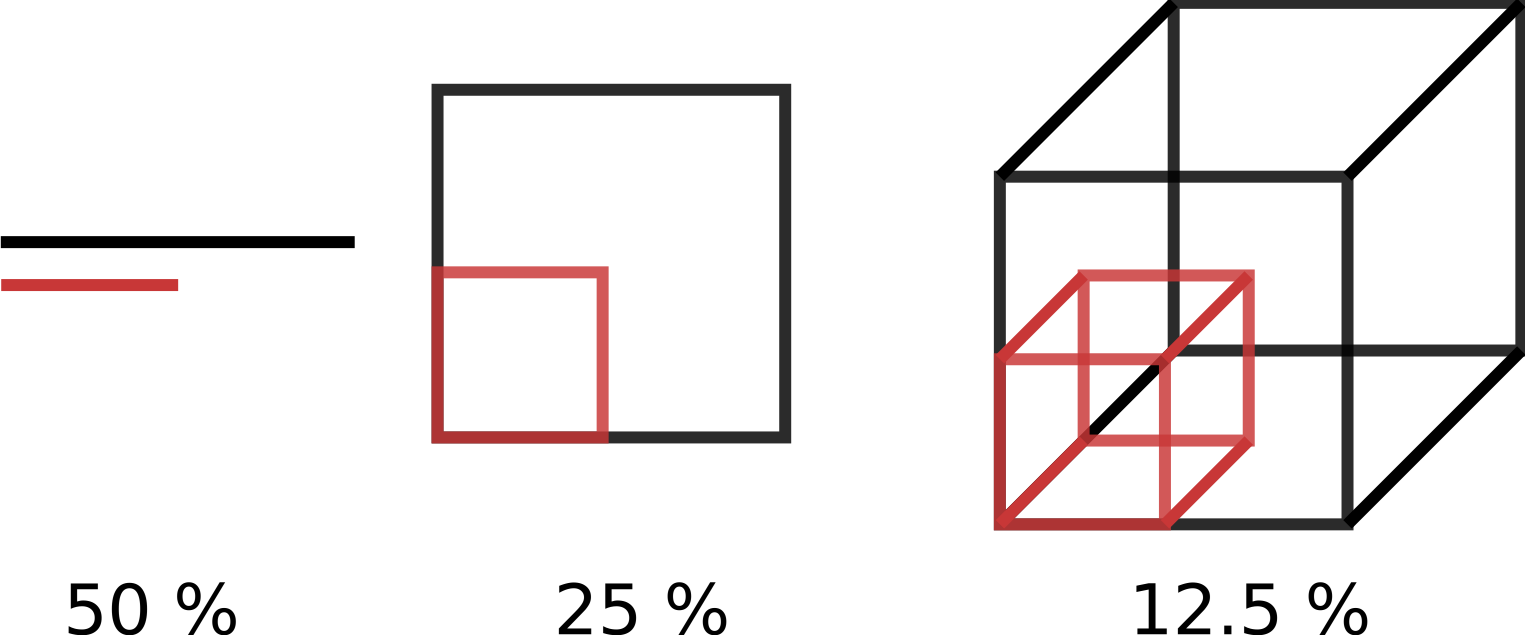
\includegraphics[height = 0.25\textheight]{images/highdimensions.pdf}
			\end{figure}
		\end{small}
	\end{enumerate}
\end{frame}


\begin{frame}{Backup - Nelder Mead algorithm}
	\metroset{block=fill}
	\begin{itemize}
		\item Every set of parameters is assigned to a scalar value by an objective function.
		\vspace{4pt}
		\item Two conditons:
		\begin{itemize}
			\item[1] The initial values must be in a stable area.
			\item[2] Optimization methods which does not need the derivative.
		\end{itemize}
		\vspace{4pt}
		\item[$\Rightarrow$] After testing several methods the downhill simplex algorithm from Nelder and Mead~\cite{NelderMead65} was chosen.
	\end{itemize}
	\begin{figure} 
		\includegraphics[height = 0.3\textheight]{images/Nelder-Mead_Himmelblau.png}
		\centering \tiny Source: Wikipedia
	\end{figure}
	\begin{exampleblock}{Advantages}
		The Nelder-Mead method  does not need the derivative and is very reliable.
	\end{exampleblock}
	
	\begin{alertblock}{Disadvantages}
		The Nelder Mead algorithm is very slow and can, like many other optimization methods, converge towards a local minimum.
	\end{alertblock}
	
\end{frame}



\begin{frame}{Backup - Phase acceptance scan}
	For the VSR project it is assumed that 0.8-1.0\,ns with 90\,\% injection efficiency is the needed to inject into the short bucket~\cite{atkinson}.
	
	\begin{minipage}{0.5 \linewidth}
		\begin{figure}
			\centering
			\includegraphics[width = 0.85\textwidth]{images/05-Phase-acceptance-V4-mai.pdf}
			\label{fig:V4-phase-scan}
		\end{figure}
	\end{minipage}
	\begin{minipage}{0.45 \linewidth}
		Phase acceptance scan with SCIDs off (May 2017):
		
		The region with injection efficiency above 90\,\% is 0.57\,ns for the V4 optics
	\end{minipage}
	
	\begin{minipage}{0.5 \linewidth}
		\begin{figure}
			\centering
			\includegraphics[width = 0.85\textwidth]{images/05-comparison-phase-acceptance_sep.pdf}
			\label{fig:comparison-phase-acceptance}
		\end{figure}
	\end{minipage}
	\begin{minipage}{0.45 \linewidth}
		Phase acceptance scan with SCIDs on (September 2017):
		
		The region with injection efficiency above 90\,\% is 0.65\,ns for the current standard user lattice and 0.45\,ns for the V4 optics
	\end{minipage}
\end{frame}


\begin{frame}{Backup - LOCO (Linear Optics from Closed Orbits)}
		\begin{itemize}
			\item[1] Measure the LOCO data (BPM response matrix, dispersion function, BPM noise)
			\item[2] Build the LOCO input file (choose a accelerator model).
			\item[3] Fit the LOCO data to the model.
		\end{itemize}
\end{frame}


\begin{frame}{Backup - The Twiss GUI}
\begin{figure}
	\centering
	\includegraphics[width = 0.65\textwidth]{images/A-screenshot-Twiss-GUI.png}
	\caption{Screenshot of the Twiss GUI}
	\label{fig:Twiss-GUI}
\end{figure}
\begin{itemize}
	\item Build with the python integrated Tkinter module in combination with matplotlib libary~\cite{matplotlib}.
	\item Change quadrupoles in the style of the control room software.
\end{itemize}
\end{frame}


\begin{frame}{Backup - Optimizing of the optics}
	\begin{minipage}{0.6 \linewidth}
		\begin{itemize}
			\item GUI can be used to choose the sets of parameters.
			\item The different fits can be configured one by one and are then computed in parallel.
			\item Afterwards the GUI can be closed without terminating the process.
		\end{itemize}
	\end{minipage}
	\begin{minipage}{0.39 \linewidth}	
		\begin{figure}
			\centering
			\includegraphics[width = \linewidth]{images/A-screenshot-Fit-GUI.png}
			\caption{Screenshot of the Fit GUI}
		\end{figure}
	\end{minipage}
\end{frame}







\begin{frame}[allowframebreaks]{References}
	\renewcommand*{\newunitpunct}{\addcomma\space} % komma statt punkt
	\printbibliography[heading=bibintoc]
\end{frame}
\end{document}  